% 
%
\documentclass[12pt]{article}
% General packages
\usepackage{amsmath, graphicx, float, tabularx, booktabs}
% For coloring tables
%\usepackage[table]{xcolor}
% For adjusting margin size
\usepackage[margin=1in]{geometry}
% For setting bookmarks on pdf export
\usepackage[bookmarks,bookmarksopen,bookmarksdepth=2]{hyperref} 
\usepackage{cite}

% Image path location
\graphicspath{ {images/} }

%\rowcolors{2}{gray!25}{white}

\begin{document}

% Title information
\title{Linear Block Code Error Correction}
\author{Devin Trejo \tabularnewline devin.trejo@temple.edu }
\date{\today}
\maketitle

\section{Summary}
\label{sect:summary}
We introduce the (6,3)~Hamming Linear Block Coding a error detecting and 
correcting algorithm. For this lab we will parse a string into 3-bit sized
messages and encoded into 6-bit codewords. We then transmit our codewords
as characters to a Windows client from a PIC32 MCU. To simulate a noisy
communication medium our client introduces random errors into our message
and returns it back to the server. We show that the Hamming LBC is capable
of correcting up to 1-bit in error for each received codeword.

\section{Introduction}
\label{sect:intro}
\subsection{Hamming Linear Block Encoding/Decoding Theory}
\label{sec:theory}
The Hamming linear block code is a forward error detection and correction 
method where the original message is encoded to include more symbols to 
add redundancy to the original message. The process allows the receiver of
the message to check and attempt to correct errors introduced by a 
noisy communications channel. In this lab we will use a (6,3)~Hamming code
generator~matrix~(G) which we will transform a 3-bit messages~($\vec{m}$) 
into 6-bit codewords~($\vec{x}$).

\begin{equation}
    \vec{x}=\vec{p}G \text{ where,}
    \label{eq:encoder}
\end{equation}

$$
    G=
    \begin{bmatrix}
        1 & 0 & 0 & 1 & 1 & 0 \\
        0 & 1 & 0 & 1 & 1 & 1 \\
        0 & 0 & 1 & 1 & 0 & 1
    \end{bmatrix} \quad
$$

On the receiving side we first take our received codeword~($\vec{r}$) and 
detect any errors in the received message. We do so by taking our 
codeword and checking it against a parity~matrix~(H). Note that our linear 
block code produces a systematic codeword; meaning our message is separated 
into k message bits and (n-k) parity bits. \cite{Balakrishnan2010} 

\begin{equation}
    \vec{z}=\vec{r}H \text{ where,}
    \label{eq:error_detector}
\end{equation}

$$
    H=
    \begin{bmatrix}
        1 & 1 & 0 \\
        1 & 1 & 1 \\
        1 & 0 & 1 \\
        1 & 0 & 0 \\
        0 & 1 & 0 \\
        0 & 0 & 1 \\
    \end{bmatrix}
$$

\begin{figure}[H]
    \centering
    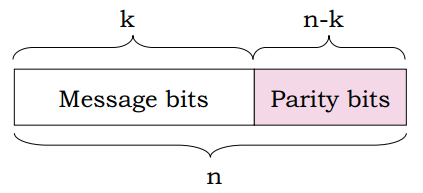
\includegraphics[width=2.5in]{systematic_encoded.PNG}
    \caption{Example of Systematic Encoding Formating
             \cite{Balakrishnan2010}}
\end{figure}

The generator~matrix~(G) is constructed from an identity matrix of size 
$k\times k$ concatenated with a matrix A of size $k\times (n-k)$ to the 
left. If we take matrix A we can create our parity~matrix~(H) by 
concatenating it with a identity matrix of size $(n-k)\times (n-k)$ on the
bottom.

$$
    G_{kxn}=
    \begin{bmatrix}
        I_{k\times k} & | & A_{k\times (n-k)}
    \end{bmatrix}
    \quad
    H_{nxk}=
    \begin{bmatrix}
        A_{k\times (n-k)} \\ I_{(n-k)\times (n-k)}
    \end{bmatrix}
$$

The error detector referenced by equation~\ref{eq:error_detector} is said to 
detect an error when the syndrome~($\vec{z}$) in non-zero.
The error correction works by correcting the bit in the received codeword in 
reference to a minimized \textbf{Hamming Distance} between a syndrome in the
set of possible valid syndromes~($\vec{z'}$) and the calculated 
syndrome~($\vec{z}$). We can calculate a set of possible valid 
syndromes~($\vec{z'}$) by multiplying the parity~check~matrix~(H) by an
identity (I); where the identity simulates codewords where one bit is flipped.
The result tells us an error in the MSB (bit-6) maps to a syndrome of 
$\vec{z}=\begin{bmatrix} 1 & 1 & 0 \end{bmatrix}$ and so on.

$$
    H=I*H=
    \begin{bmatrix}
        1 & 0 & 0 & 0 & 0 & 0 \\
        0 & 1 & 0 & 0 & 0 & 0 \\
        0 & 0 & 1 & 0 & 0 & 0 \\
        0 & 0 & 0 & 1 & 0 & 0 \\
        0 & 0 & 0 & 0 & 1 & 0 \\
        0 & 0 & 0 & 0 & 0 & 1 \\
    \end{bmatrix}
    *
    \begin{bmatrix}
        1 & 1 & 0 \\
        1 & 1 & 1 \\
        1 & 0 & 1 \\
        1 & 0 & 0 \\
        0 & 1 & 0 \\
        0 & 0 & 1 \\
    \end{bmatrix}
$$

After we have our codeword corrected ($\vec{r'}$), we can retrieve the 
original message ($\vec{p_r}$) by using a (3,6) decoding~matrix~(R). 
The decoding matrix reverses the steps taken by the generator~matrix~(G). 

\begin{equation}
    \vec{p_r}=\vec{r'}R \text{ where, }
    \label{eq:decoder}   
\end{equation}

$$
    R=
    \begin{bmatrix}
        1 & 0 & 0 \\
        0 & 1 & 0 \\
        0 & 0 & 1 \\
        0 & 0 & 0 \\
        0 & 0 & 0 \\
        0 & 0 & 0 \\
    \end{bmatrix}
$$

Finally we wish to look at the performance of this Hamming Linear Block code
encoder/decoder. The correction capacity for any given codeword is given by
equation~\ref{eq:correction_capacity} where t denotes the number of 
errors that are detectable and correctable. In some instances the receiver may
not be able to correct a received codeword but it is still detectable. 
The error detection~(e) is given by equation~\ref{eq:error_detection}.

\begin{equation}
    t=\lfloor{\frac{d_{min}-1}{2}}\rfloor
    \label{eq:correction_capacity}   
\end{equation}

\begin{equation}
    e={d_{min}-1}
    \label{eq:error_detection}   
\end{equation}

\subsection{Hamming Linear Block Encoding/Decoding Implementation}
\label{sec:implementation}
For this lab we will transmit the message \textit{``EE is my avocation''} 
and set up a communication channel between a PIC32 Microchip MCU and 
Windows desktop over Ethernet. The Windows machine will run a Visual Basic 
application which will receive a message from the PIC32 server and 
introduce random errors to simulate errors that may be introduced
when transmitting over a noisy communications channel. VB client \
\textit{Client2 v16B} will introduce at most 1-bit in error within a given
message. VB Client \textit{Client3 v16} will introduce up to 10-bits in 
error. After we will setup our PIC32 MCU to receive a message from the VB 
client in order to perform error detection and correction using the Hamming 
linear block scheme.

To use a (6,3)~Hamming~code requires our individual messages to be 3-bits in
size. Therefore, we format our transmission string into messages 3-bits in 
size. We then will encode our message to produce 6-bit codewords. Since
our message is using characters within the standard ASCII table, the MSB in 
all characters will always be zero. Therefore, ignoring the MSB can now take 
our 7-bit ASCII character and break it up 3 individual bits. A combination 
of 3 characters will end up creating a perfect set to complete 7 packets 
we can send. 

$$
    \begin{array}{ccccc}
        'E' & = & [ 0 1 0 0 \quad 0 1 0 1] 
                & \rightarrow & [ 1 0 0 \quad 0 1 0 1] \\
        'E' & = & [ 0 1 0 0 \quad 0 1 0 1] 
                & \rightarrow & [ 1 0 0 \quad 0 1 0 1] \\
        '\text{\textvisiblespace }' & = & [ 0 1 0 0 \quad 0 0 0 0] 
                                    & \rightarrow
                                    & [ 1 0 0 \quad 0 0 0 0 ]
    \end{array}
$$

\begin{table}[H]
    \centering
    \begin{tabularx}{\textwidth}{|*{7}{>{\centering}X|}}
        \toprule
        100 & 010 & 110 & 001 & 011 & 000 & 000 \tabularnewline
        \midrule
        \multicolumn{1}{|c|}{\textit{\textbf{$\vec{p_0}$}}} & 
        \multicolumn{1}{|c|}{\textit{\textbf{$\vec{p_1}$}}} & 
        \multicolumn{1}{|c|}{\textit{\textbf{$\vec{p_2}$}}} & 
        \multicolumn{1}{|c|}{\textit{\textbf{$\vec{p_3}$}}} & 
        \multicolumn{1}{|c|}{\textit{\textbf{$\vec{p_4}$}}} & 
        \multicolumn{1}{|c|}{\textit{\textbf{$\vec{p_5}$}}} & 
        \multicolumn{1}{|c|}{\textit{\textbf{$\vec{p_6}$}}} \tabularnewline
        \bottomrule
    \end{tabularx}
    \caption{3-Bit Message Composition for First 3 Characters}
    \label{table:3-bit_messages}   
\end{table}

Our overall message is 18 characters in length. Distributing our 18 
characters into 7 packets of length 3-bits produces 42 packets.
Those 42 packets will next be encoded using our (6,3)~Hamming 
linear block encoder to produce packets of 6-bits. Finally, we will 
pad each 6-bit packet with two leading zeros and send it as a 8-bit ASCII 
character. The final transmitted packet sequence for the first 3 characters 
are shown in table~\ref{table:6-bit_packets_encoded} by applying 
equation~\ref{eq:encoder}.

\begin{table}[H]
    \centering
    \begin{tabularx}{\textwidth}{|*{7}{>{\centering}X|}}
        \toprule
        0010 0110 & 0001 0111 & 0011 0001 & 
        0000 1101 & 0001 1010 & 0010 0110 & 0000 0000 \tabularnewline
        \midrule
        \multicolumn{1}{|c|}{\textit{\textbf{$\vec{x_0}$}}} & 
        \multicolumn{1}{|c|}{\textit{\textbf{$\vec{x_1}$}}} & 
        \multicolumn{1}{|c|}{\textit{\textbf{$\vec{x_2}$}}} & 
        \multicolumn{1}{|c|}{\textit{\textbf{$\vec{x_3}$}}} & 
        \multicolumn{1}{|c|}{\textit{\textbf{$\vec{x_4}$}}} & 
        \multicolumn{1}{|c|}{\textit{\textbf{$\vec{x_5}$}}} & 
        \multicolumn{1}{|c|}{\textit{\textbf{$\vec{x_6}$}}} \tabularnewline
        \bottomrule
    \end{tabularx}
    \caption{6-Bit Codewords Composition for First 3 Characters}
    \label{table:6-bit_packets_encoded}   
\end{table}

\section{Discussion}
\label{sect:discussion}

To begin we need several functions that will allows us to create our 
As will be seen in order to analyze our experiments, we send
the PIC32 MCU server a a return message back. The returned message may
have errors randomly distributed throughout as to simulate a noisy 
communications channel. The server will receive the message and detect 
and attempt to correct any errors. With the code provided 
(see Appendix) a uncorrectable error will light up
the PIC32's red LED (LED0). A correctable error will flash the PIC32's
yellow LED (LED1) as it goes about correcting any errors. 

We can use WireShark to analyze the packet transmitted from our server 
PIC32 MCU to our VB client. We expect the first seven packets to be as 
demonstrated in table~\ref{table:6-bit_packets_encoded}. The 42 packets
that make up our overall transmission can be seen in highlighted
figure~\ref{fig:piccontrol}. 

\begin{figure}[H]
    \centering
    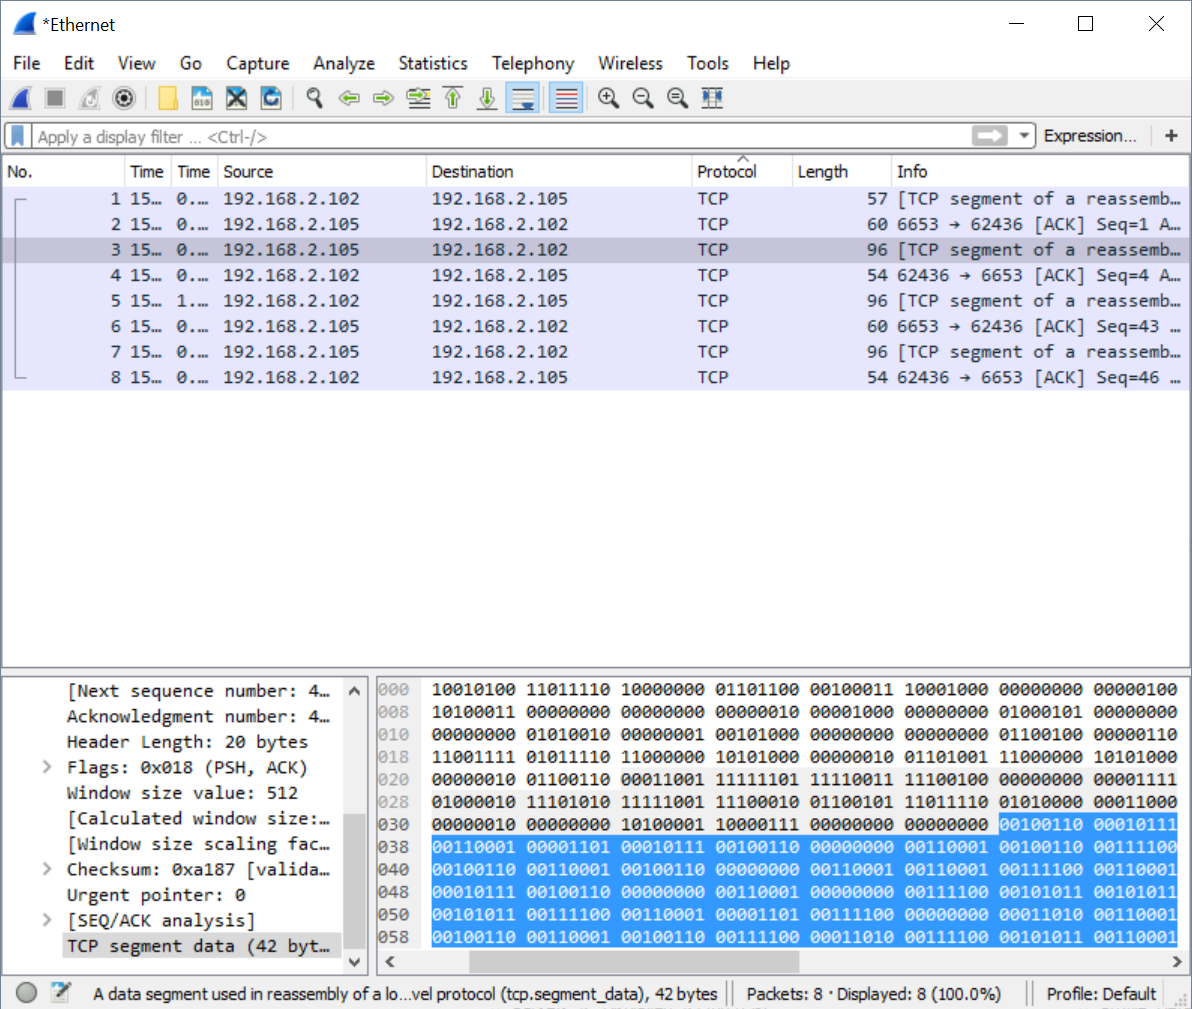
\includegraphics[width=5.5in]{images/wireshark_source_tx.PNG}
    \caption{WireShark Capture of 42 Packets Tx 
        PIC32 MCU $\rightarrow$ Windows Desktop}
    \label{fig:piccontrol}
\end{figure}

\subsection{Control Case: No Errors Introduced}
\label{sec:control}

Next we want to ensure decoding of a message with no errors introduced 
works as designed. The expected transmitted message from the 
Windows Desktop with no errors will be the same
as that seen when the message was initially transmitted to the Windows Desktop
client referenced by figure~\ref{fig:piccontrol}. As can be seen 
in the transmitted message from the Windows Desktop client, no errors were 
introduced.

\begin{figure}[H]
    \centering
    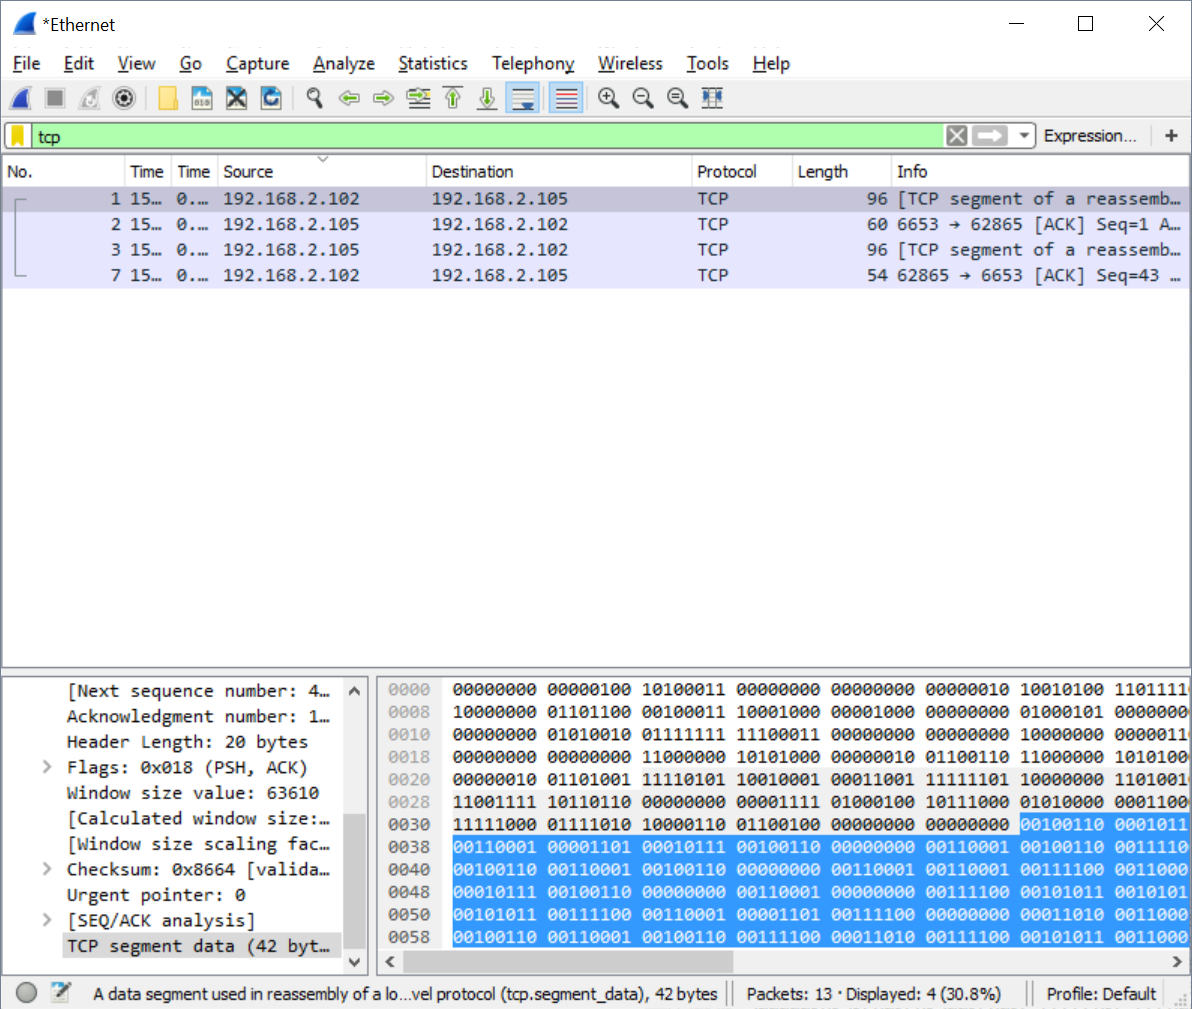
\includegraphics[width=5.5in]{images/wireshark_vbtx_noerror_packets.PNG}
    \caption{WireShark Capture of 42 Packets Tx 
        Windows Desktop $\rightarrow$ PIC32 MCU with No Error}
    \label{fig:vbnoerror}
\end{figure}

The message echoed by the PIC32 server should be the same as that transmitted
to it since there were no errors introduced. Comparing figure~\ref{fig:vbnoerror} 
with figure~\ref{fig:picnoerror} we can see no discrepancies. 

\begin{figure}[H]
    \centering
    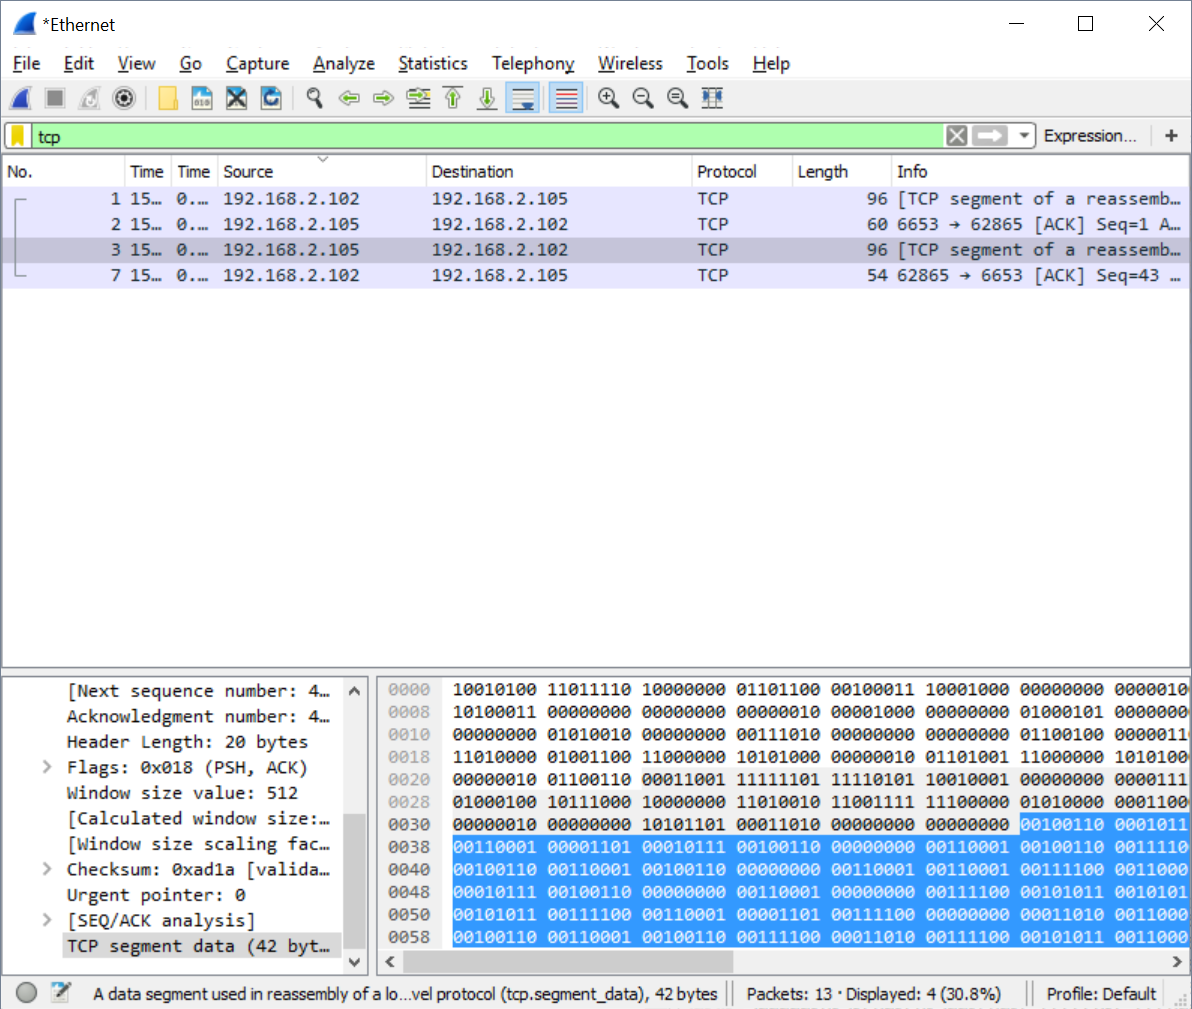
\includegraphics[width=5.5in]{images/wireshark_pictx_noerror_packets.PNG}
    \caption{WireShark Capture of 42 Packets Tx 
        PIC32 MCU $\rightarrow$ Windows Desktop with No Error}
    \label{fig:picnoerror}
\end{figure}

\subsection{1-Bit Error}
\label{sec:1biterror}

Next we show that for one bit in error our Hamming error detector and 
corrector will be able to detect any introduced errors. The error in
this 1-bit error test was introduced into the 48th row of the 
transmission. A 8-bit sequence of 0x00 was converted to 0x01. 

\begin{figure}[H]
    \centering
    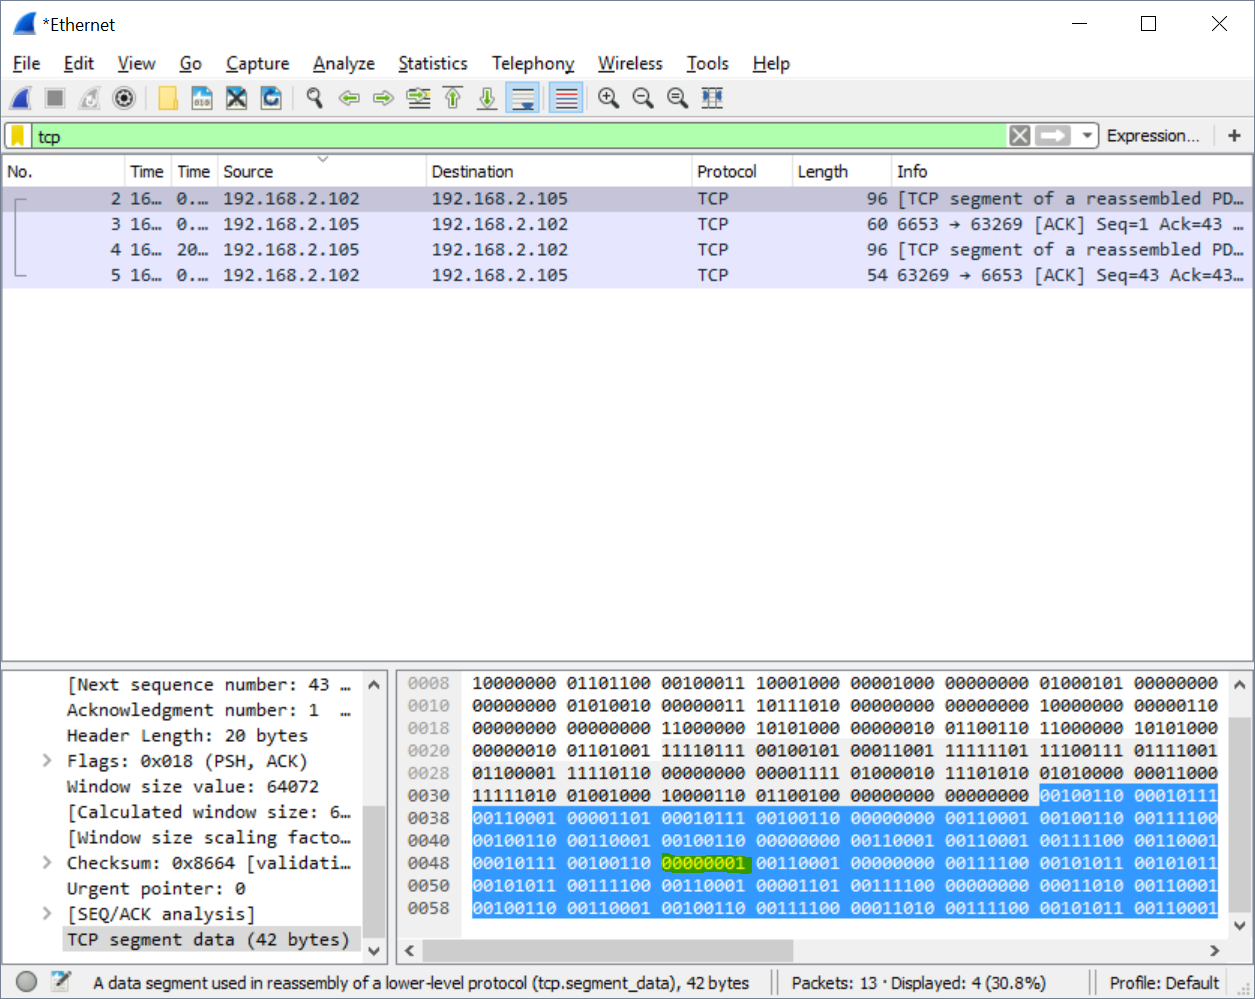
\includegraphics[width=5.5in]{images/wireshark_vbtx_1bit_packets.PNG}
    \caption{WireShark Capture of 42 Packets Tx 
        Windows Desktop $\rightarrow$ PIC32 MCU with 1-Bit Error}
    \label{fig:vb1error}
\end{figure}

The error highlighted in figure~\ref{fig:vb1error} can be seen corrected
in the echoed message from the PIC32. In reality this introduced error
effected one of the parity bits so our original message was still intact, but
the test shows that LBC can even correct errors in the parity portion of
a transmission. 

\begin{figure}[H]
    \centering
    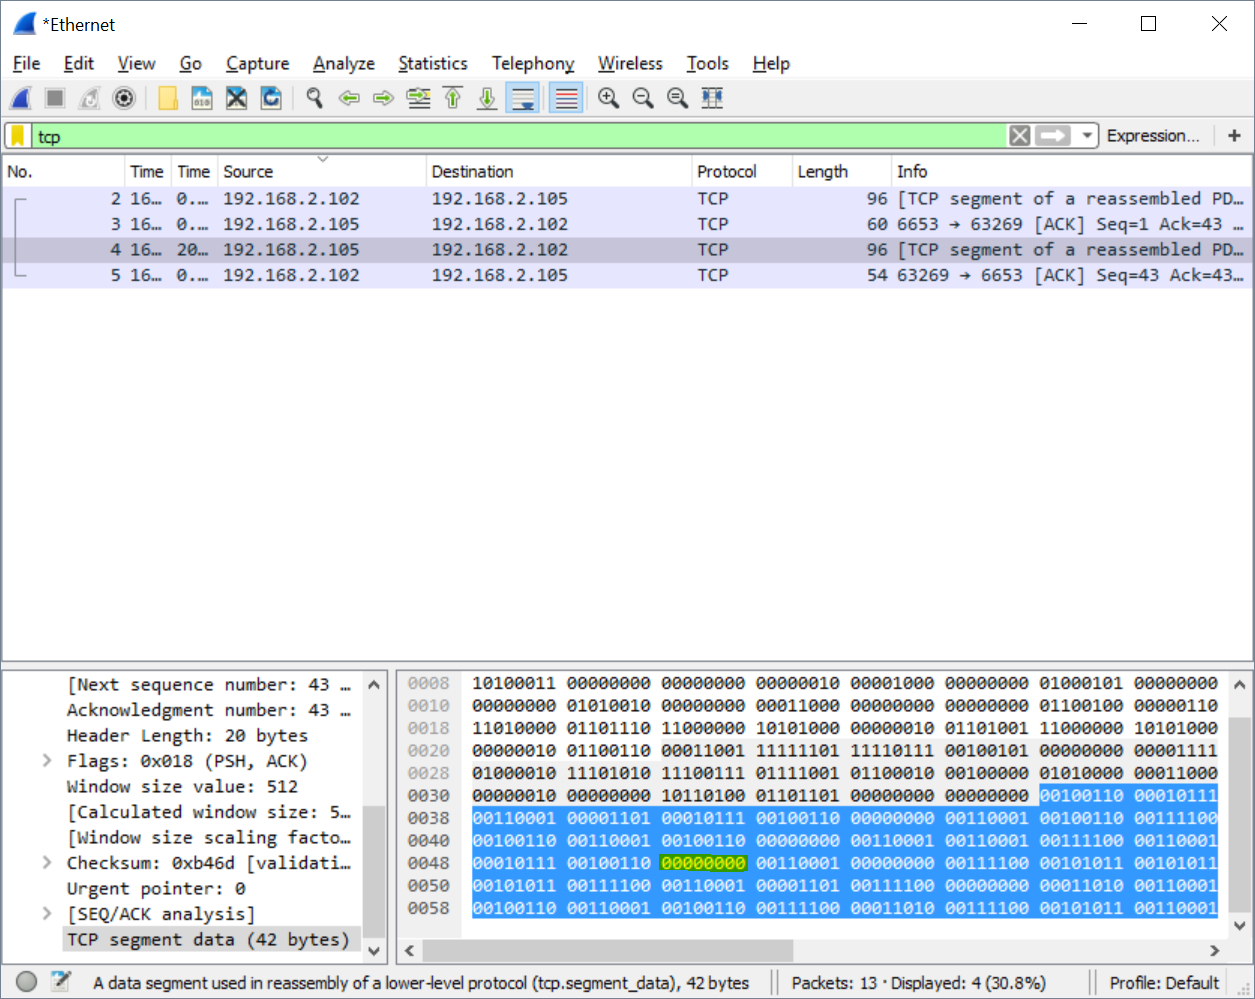
\includegraphics[width=5.5in]{images/wireshark_pictx_1bit_packets.PNG}
    \caption{WireShark Capture of 42 Packets Tx 
        PIC32 MCU $\rightarrow$ Windows Desktop with 1-Bit Error}
    \label{fig:pic1error}
\end{figure}

\subsection{Multiple Errors in Transmission}
\label{sec:multierrors}

Our last test will show that in extreme cases where more than one bit 
in error in introduced to our transmission, our Hamming decoder has the
capability to correct the error. In the next example we introduce 8 bit in
error to the packet. There are two bit errors that occur in the two MSB of
the packet. Recall that the two MSB are padded zeros, so these bit errors
are ignored.

\begin{figure}[H]
    \centering
    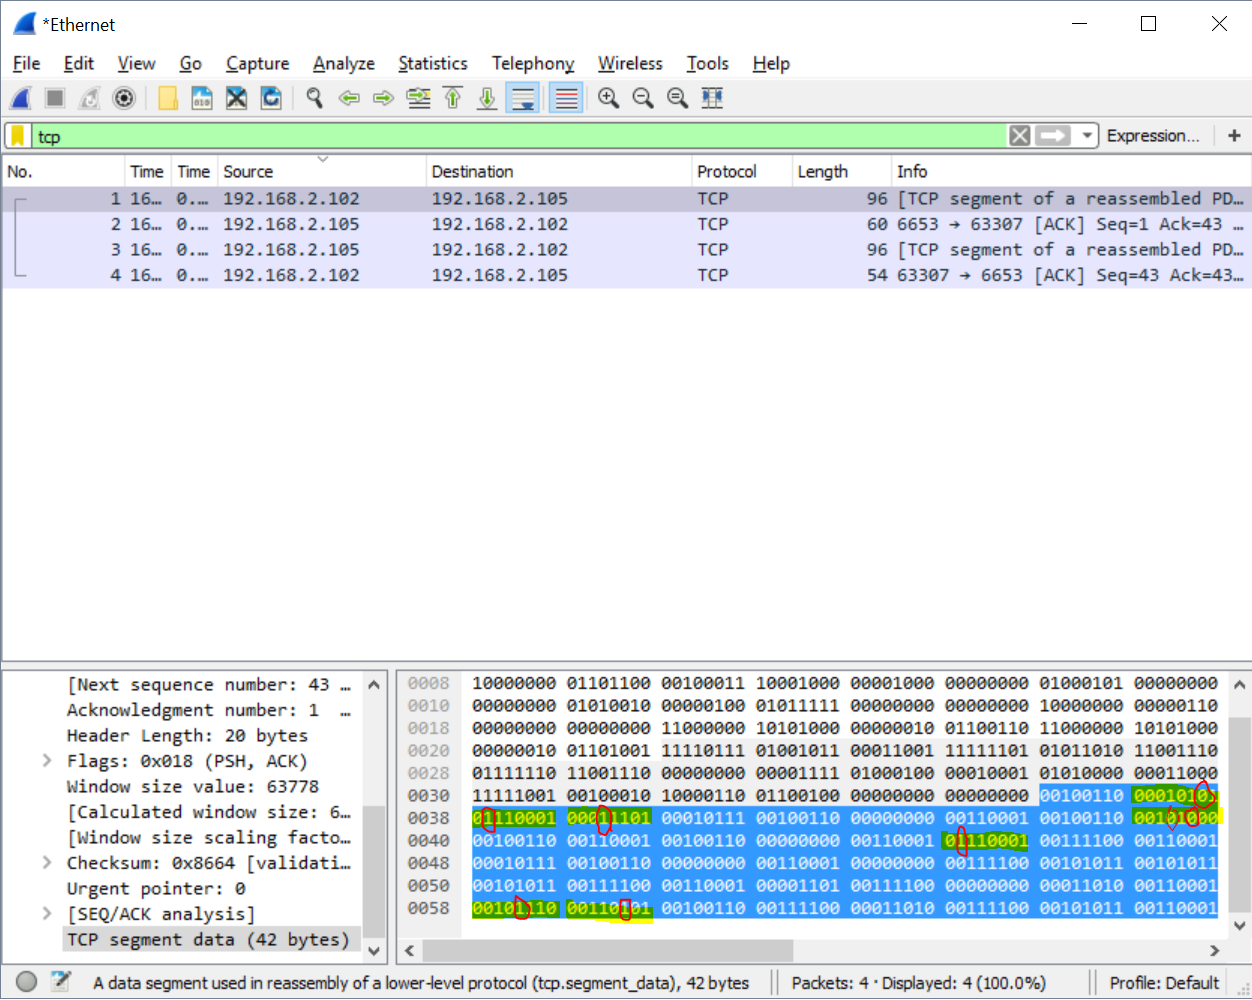
\includegraphics[width=5.5in]{images/wireshark_vbtx_multibit_packets.PNG}
    \caption{WireShark Capture of 42 Packets Tx 
        Windows Desktop $\rightarrow$ PIC32 MCU with 8-Bit Errors}
    \label{fig:vb8error}
\end{figure}

The corrected message sent echoed by the server corrects the issues it could. 
In the second byte, we can see how the second bit from the left was corrected
back to a binary 1. Our third highlighted error was also corrected so it
incorrect bit was flipped. Our forth byte sequence which contained an error
was changed to all zeros. These is behavior coded for when an error is
detected but could not be corrected. Since there were more than one bit and
error in the message the receiver could  not correct the message. In this
scenario typically we would have the receiver re-transmit the message. 

\begin{figure}[H]
    \centering
    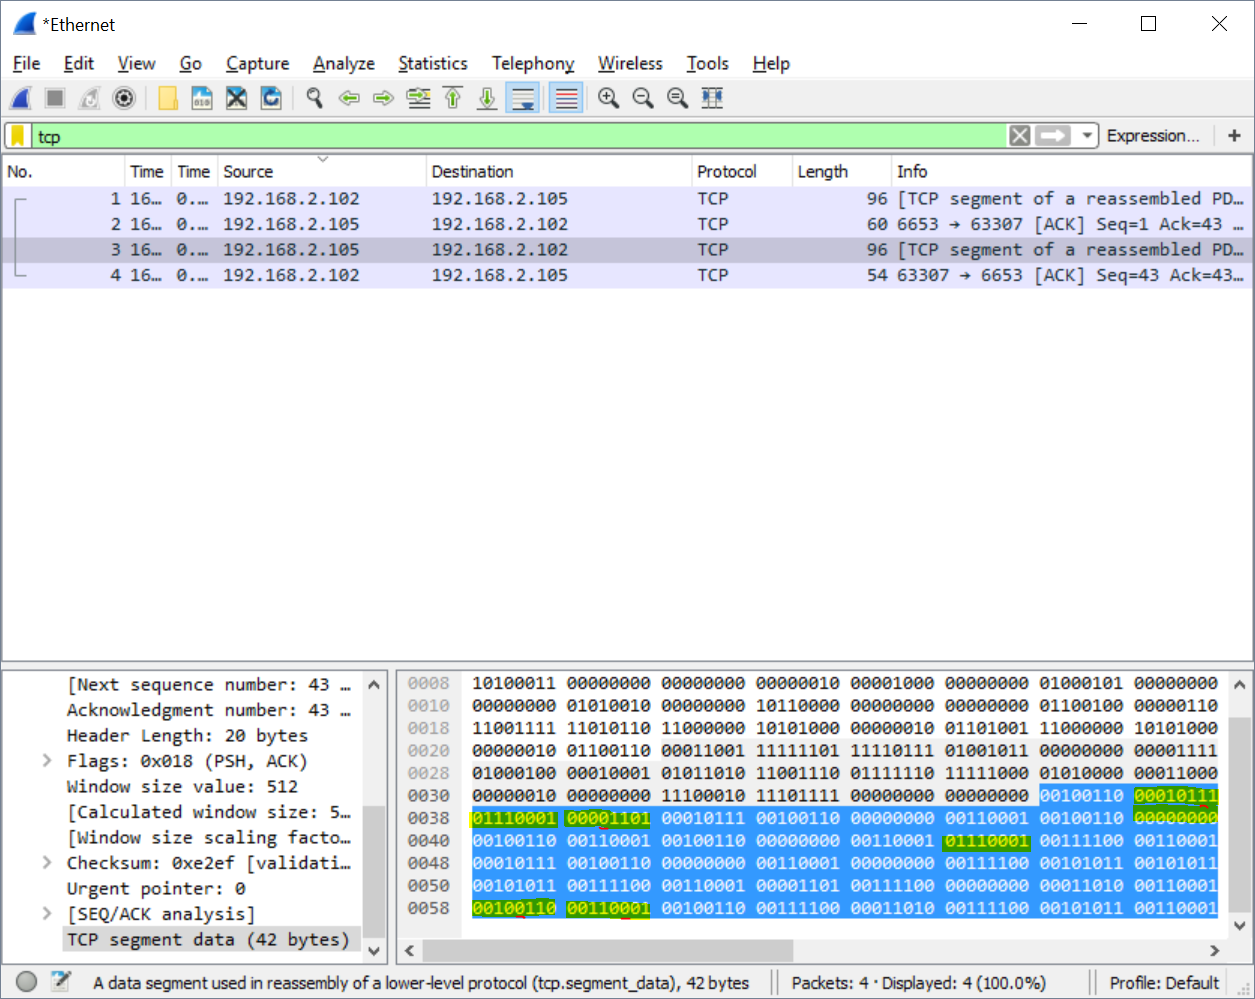
\includegraphics[width=5.5in]{images/wireshark_pictx_multibit_packets.PNG}
    \caption{WireShark Capture of 42 Packets Tx 
        PIC32 MCU $\rightarrow$ Windows Desktop with 8-Bit Errors}
    \label{fig:pic8error}
\end{figure}

As is seen in the two byte sequences that contained errors in the higher two
MSB locations, our implementation is not at its peak efficiency. 
Hypothetically our message size is $k=3$ and our codeword size is $n=6$, 
we can say out $\text{\textbf{code rate}} =\frac{k}{n} = \frac{6}{3} = 
\frac{1}{2}$. However, since we pad our codeword with two leading zeros it 
can be said that our code rate decreases to $\text{code rate} = \frac{3}{8}$.

The padding of zeros only causes our data rate to decrease. A way we could
improve our Hamming linear block encoder/decoder is by fully utilizing the 
entire length of our 8-bit packets. It will complicate the decoding process
since it would require that we extract bits from other various packets to 
construct our codeword.

\section{Conclusion}
\label{sect:conclusion} 
We have introduce another form of error detection and correction that has 
been proven to correct up to one in error. The Hamming linear block code 
are useful in forwarding error correction to reduce the need for 
retransmission of data corrupted by the transmission medium. The technique 
is effective in correcting a message in its use of codewords which convert
a message a sequence where the difference between each codeword is at least
two bits. By maximizing the between messages we can improve the performance
of this error detection and correction scheme.

\bibliographystyle{plain}
\bibliography{../../../Mendeley/data_computer_communications}

\section*{Appendix}
\label{sect:appendix}
Main program source code available on my GitHub: \\
\url{https://github.com/dtrejod/myece4532/blob/master/lab4/ECE4532%20PIC32%20BSD%20Server/source/main.c}
\end{document}